
Systematic uncertainties may change the derived limits. Uncertainties
that we consider may change the normalization or distort the shape
that we used for fits. The following sources of the uncertainties have
been included:
\begin{itemize}

 \item {\bf Luminosity}: an uncertainty of $2.5\%$ is assigned for
   2016 luminosity. All the processes are affected except those, which normalization is determined using data driven methods: DY and \ttbar normalization

 \item {\bf Lepton Efficiency}: identification, isolation, tracker,
   and trigger scale factors have been determined using the standard EGamma POG and Muon POG technique of the Tag-and-Probe. 
   Up and Down variations with respect to the nominal value of the scale factor (within the uncertainty on the value) have been propagated to the final HH transverse mass shape that goes to the fit with the Higgs Combination Tool. Each scale factor type (identification, isolation, tracker,
   and trigger scale factor) is propagated independently. Overall, the effect of the lepton efficiency, when dealing with b jets, is a very minor
   one.  These uncertainties are included in both electron and muon channels.

 \item {\bf MET}: the effect of the JEC and JER on the MET is studied modifying MET variables that go into HH transverse mass shape used in the final fit. The effect of the calibration of unclustered MET, meaning missing energy associated with particles that are not clustered into jets, is found only on the normalization, the shape itself is not distorted. The size of the effect is $~3\%$ depending on the mass hypothesis and the $3\%$ normalization uncertainty is used in the analysis.

 \item {\bf Jet Energy Scale}: following JetMET group recommendation we check the effect of this uncertainty
   on all jet-related variables that enter BDT and/or HH system. The scale value is varied Up and Down and modified HH
   transverse mass shapes are obtained and used in the final fit.

 \item {\bf Jet Energy Resolution}: we vary up and down jet energy
   resolution by one $\sigma$ and modify all the jet related
   variables that are a part of the BDT and/or HH system prior to constructing the final shape. Varied HH transverse mass shapes are used in the final fit.

 \item {\bf B-jet Tagging and mistag uncertainties}: following the suggestions from the BTV POG
   b tag and mistag scale factors are applied to all MC samples. The effect of the usage of 
   light and heavy flavor scale factors is propagated to the final shapes.

 %% \item {\bf PDF uncertainties}: impossibility to know precisely the
 %%   content of the colliding proton or gluon is addressed in this
 %%   uncertainty. Using the recommended values from LHC Higgs Cross Section group documented in the CERNYellowReportPageAt13TeV we assign $O(1-5)\%$ uncertainties to quark-quark initiated
 %%   processes and $O(10-20)\%$ uncertainties to gluon-gluon uncertainties depending on the process.
  
 %% \item {\bf QCD scale variations}: The uncertainty on the QCD normalization scale for each
 %%   individual process is assigned to a corresponding specific theory error suggested by CMS generator group, which maintains a twiki page with a collection of cross sections for Standard Model processes to be used in the CMS analyses. More information on how the cross-sections and the associated theory errors have been determined is available at ~\cite{SMxsec}. 

\item {\bf QCD scale variations}: This uncertainty is estimated by varying the renormalization ($\mu_{R}$) and the factorization ($\mu_{F}$) scales, independently by a factor of 2, meaning from the nominal value of 1 to values of 0.5 and 2. Unphysical situations with one scale fluctuating up and the other fluctuating down are not considered. In each bin of the distribution the maximum (minimum) variation is used as an estimate of the QCD scale uncertainties for all the background and signal samples. The resulting effect has been found on the normalization at the order of $4-6\%$.


\item {\bf PDF uncertainties}: impossibility to know precisely the
   content of the colliding proton or gluon is addressed in this
   uncertainty. The RMS of each of the 101 NNPDF MC variations of the strong coupling constant for each simulated background and signal processes is calculated and the largest one is assigned as a normalization uncertainty, and is of the order of $5\%$. 





%% \item {\bf PDF uncertainties}: impossibility to know precisely the
%%    content of the colliding proton or gluon is addressed in this
%%    uncertainty. For each process, the RMS of each of the 101 NNPDF MC variations is calculated and the largest one is assigned as a normalization un\
%% certainty, and is of the order of $5\%$.

%%  \item {\bf QCD scale variations}: The QCD scale normalization and factorization at $1/2$ and 2 have been applied to each sample and the resulting e\
%% ffect has been found to be $4-6\%$.





 %\item {\bf Cross section normalization}: Uncertainty associated with the cross section value for the
   %\ttbar and single top processes. We used the same numbers as in bbVV analysis.

 \item {\bf Pile up }: The effect of pile up on each
   process is considered. The recommended nominal value of 69.2 mb is used for the total inelastic pp cross section, for Down and Up variations, the values of 66.02 and 72.38 mb are used respectively. The effect is seen only in the normalization and we, thus, switch to the normalization uncertainty and assign the value of $6\%$.


 \item {\bf Drell-Yan and \ttbar normalizations }: \ttbar and Drell-Yan
   normalizations we extract from the simultaneous fit of both signal
   region and DY and \ttbar ~control regions. Normalizations of main backgrounds are allowed to float freely to let the fitter find the best values of the DY and \ttbar normalizations to fit the existing data. HH transverse mass distributions are used in the fit. Separately, an option of control regions only fit has been studied and results were found consistent with the DY and \ttbar normalizations obtained from the fit where signal region was included. Overall, the normalization of \ttbar is near the value
   '1', deviating up to $\approx10-20\%$ depending on the mass point. DY normalization is deviating higher from the value of '1' since the requirement on 2 b jets and a high boost pushes DY process to higher pT and flavor phase space that is not well modeled in the MC. Therefore, a part of the analysis strategy was to extract these numbers using the real data. The final $\chi^2$ values after the application of \ttbar and Drell-Yan normalizations are near the value '1'.

 \item {\bf Bin-by-bin uncertainties } To account for the low statistics in some bins of HH transverse mass distribution in MC, bin-by-bin uncertainties should be used. If the error on the MC in the bin is zero, the bin is skipped entirely. However, if the error is non zero and if the number of effective events for each given process is lower than or equal to zero, a Poisson-constrained parameter will be created. Otherwise a Gaussian-constrained parameter is assigned to this bin. Barlow-Beeston algorithm is used to create these bin-by-bin parameters which scale the total yield in the bin. The advantage of this algorithm is that each nuisance parameter has a simple analytic form and analytic minimization can be performed, which results in the reduction of the fit time and an increase of the fit stability.

 \item {\bf Shape uncertainties}: All shape systematic
   uncertainties are addressed separately and all together are used in the final fit. The following uncertainties are considered as shape
   uncertainties: each of lepton scale factors, b tag scale factors of
   both light and heavy flavour, effect of JEC and JER on all the variables used in
   BDT and/or HH system. For all these shape uncertainties we
   propagate the source of uncertainty through all the related
   variables that enter our BDT or region selection all the way to
   building the HH candidate and obtaining the final shape.  We
   produce, therefore, final shapes with the 'nominal value' as well
   as with 1~$\sigma$ 'Up' and 'Down' variations. 

\end{itemize}


%% \begin{center}
%% \begin{figure}[tbp]
%% %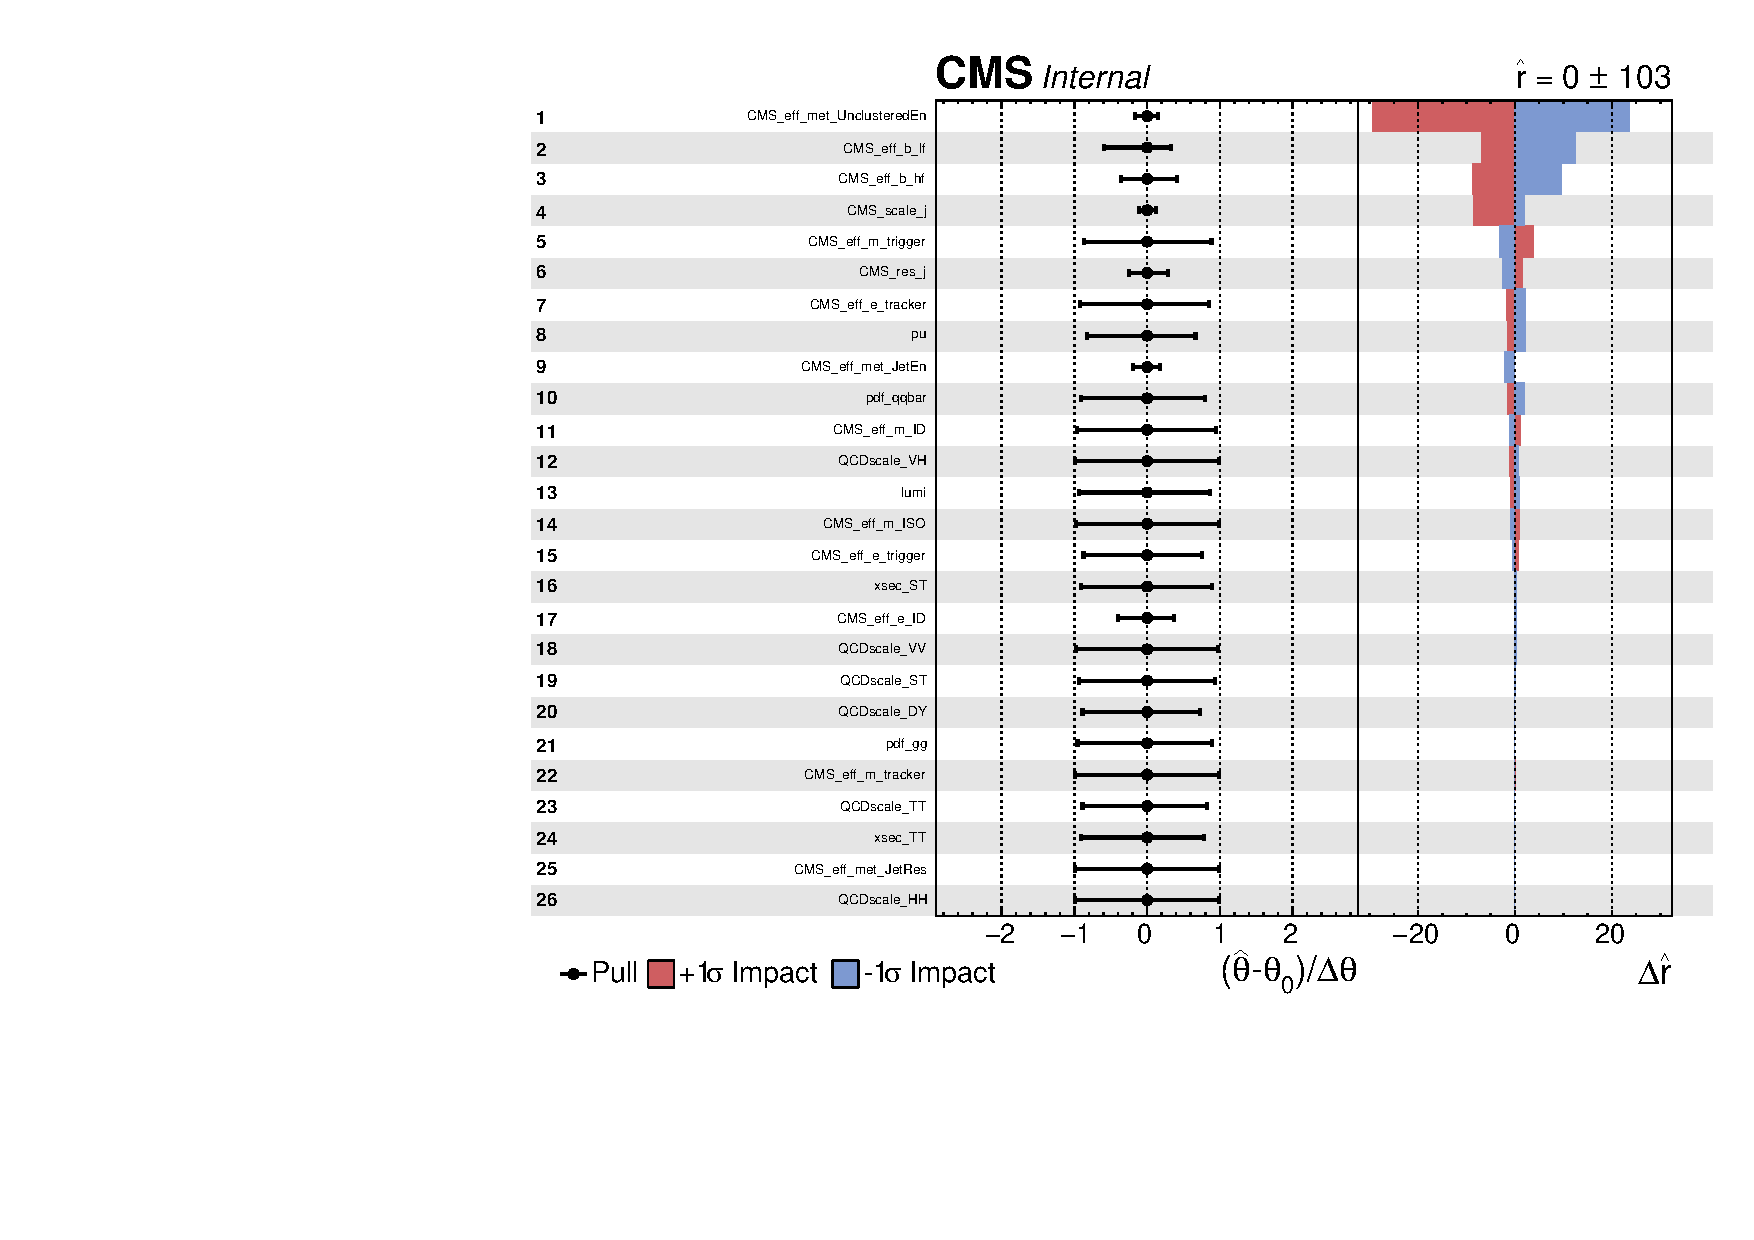
\includegraphics[width=0.5\textheight]{figures/impacts_nov7_300GeV.pdf}
%% %\caption{ Impacts plot for 300 GeV case. Actual limit at this mass point is $248.25_{-71.07}^{+103.9}$~pb.}
%% %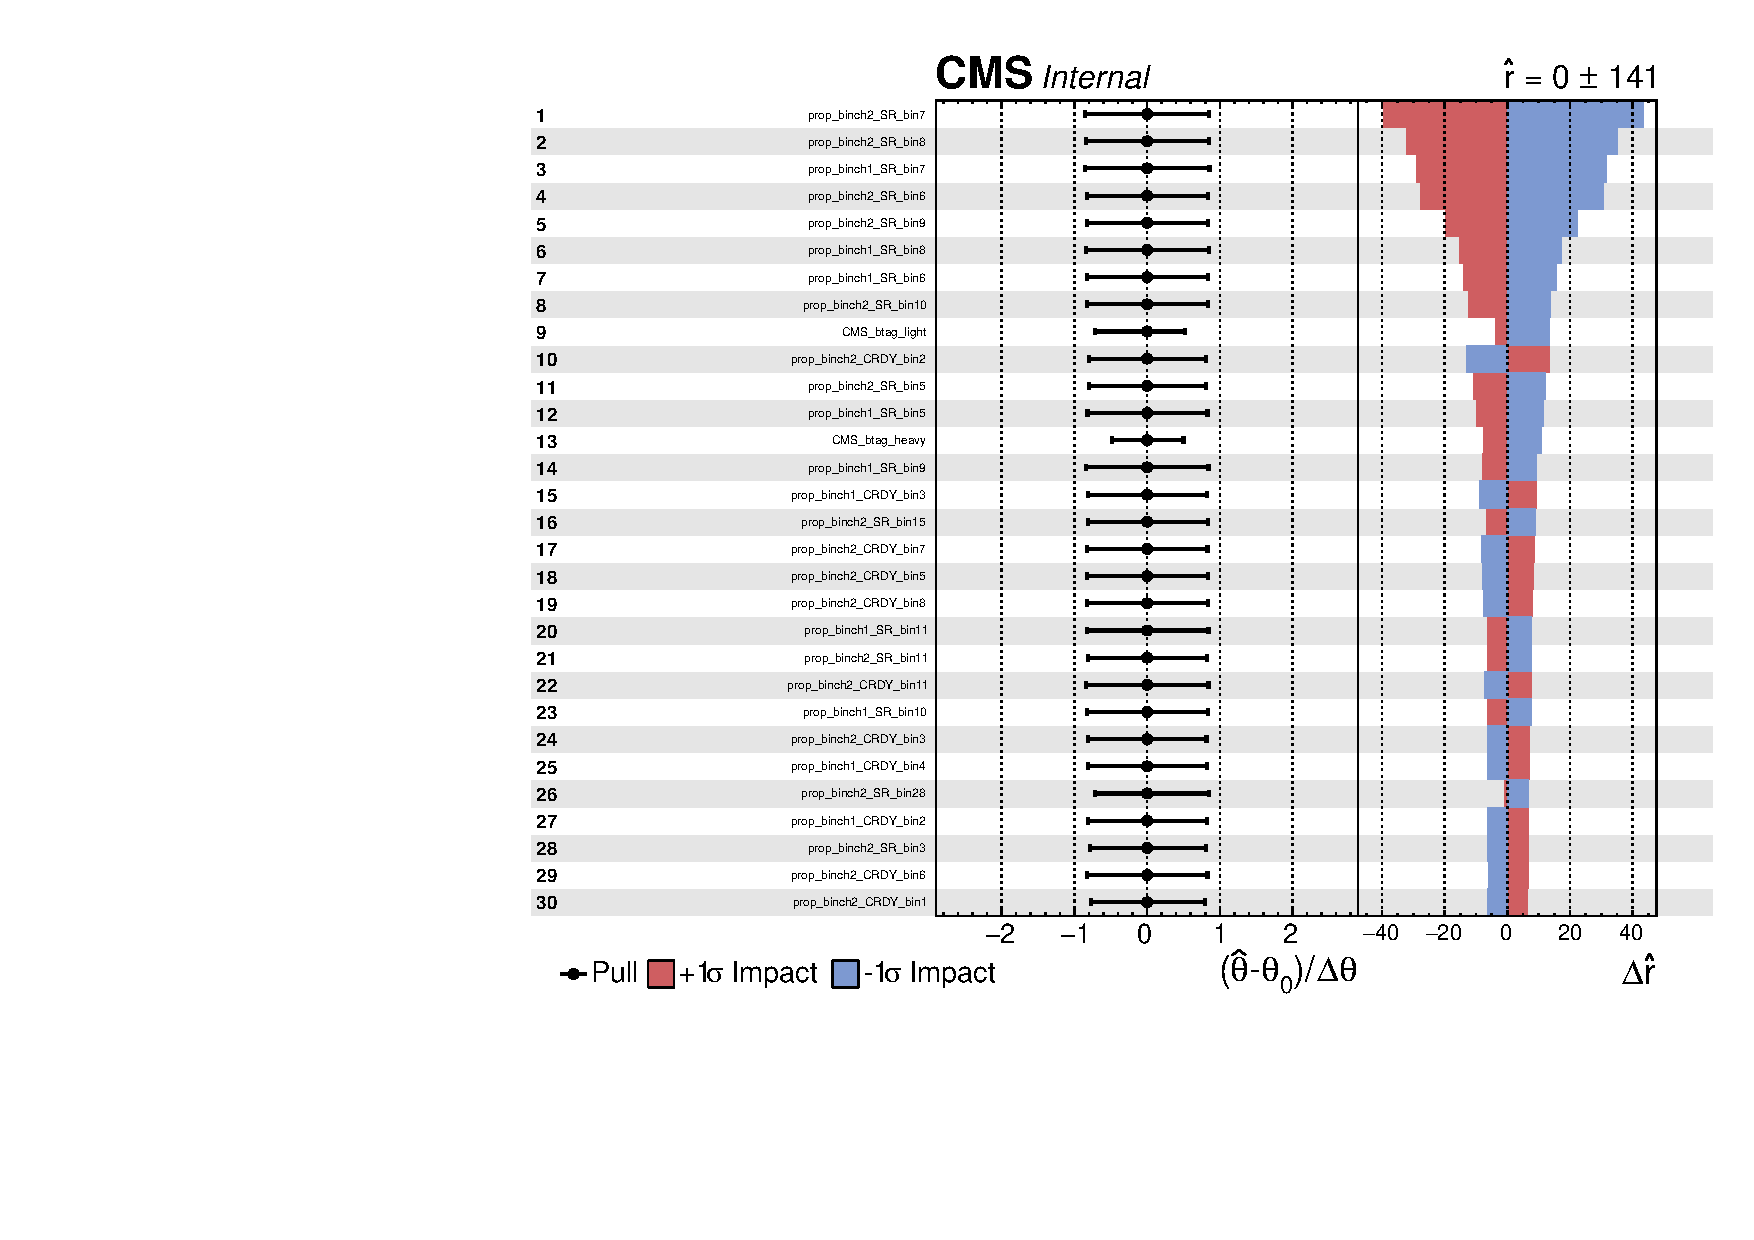
\includegraphics[width=0.5\textheight]{figures/impacts_april6.pdf}
%% 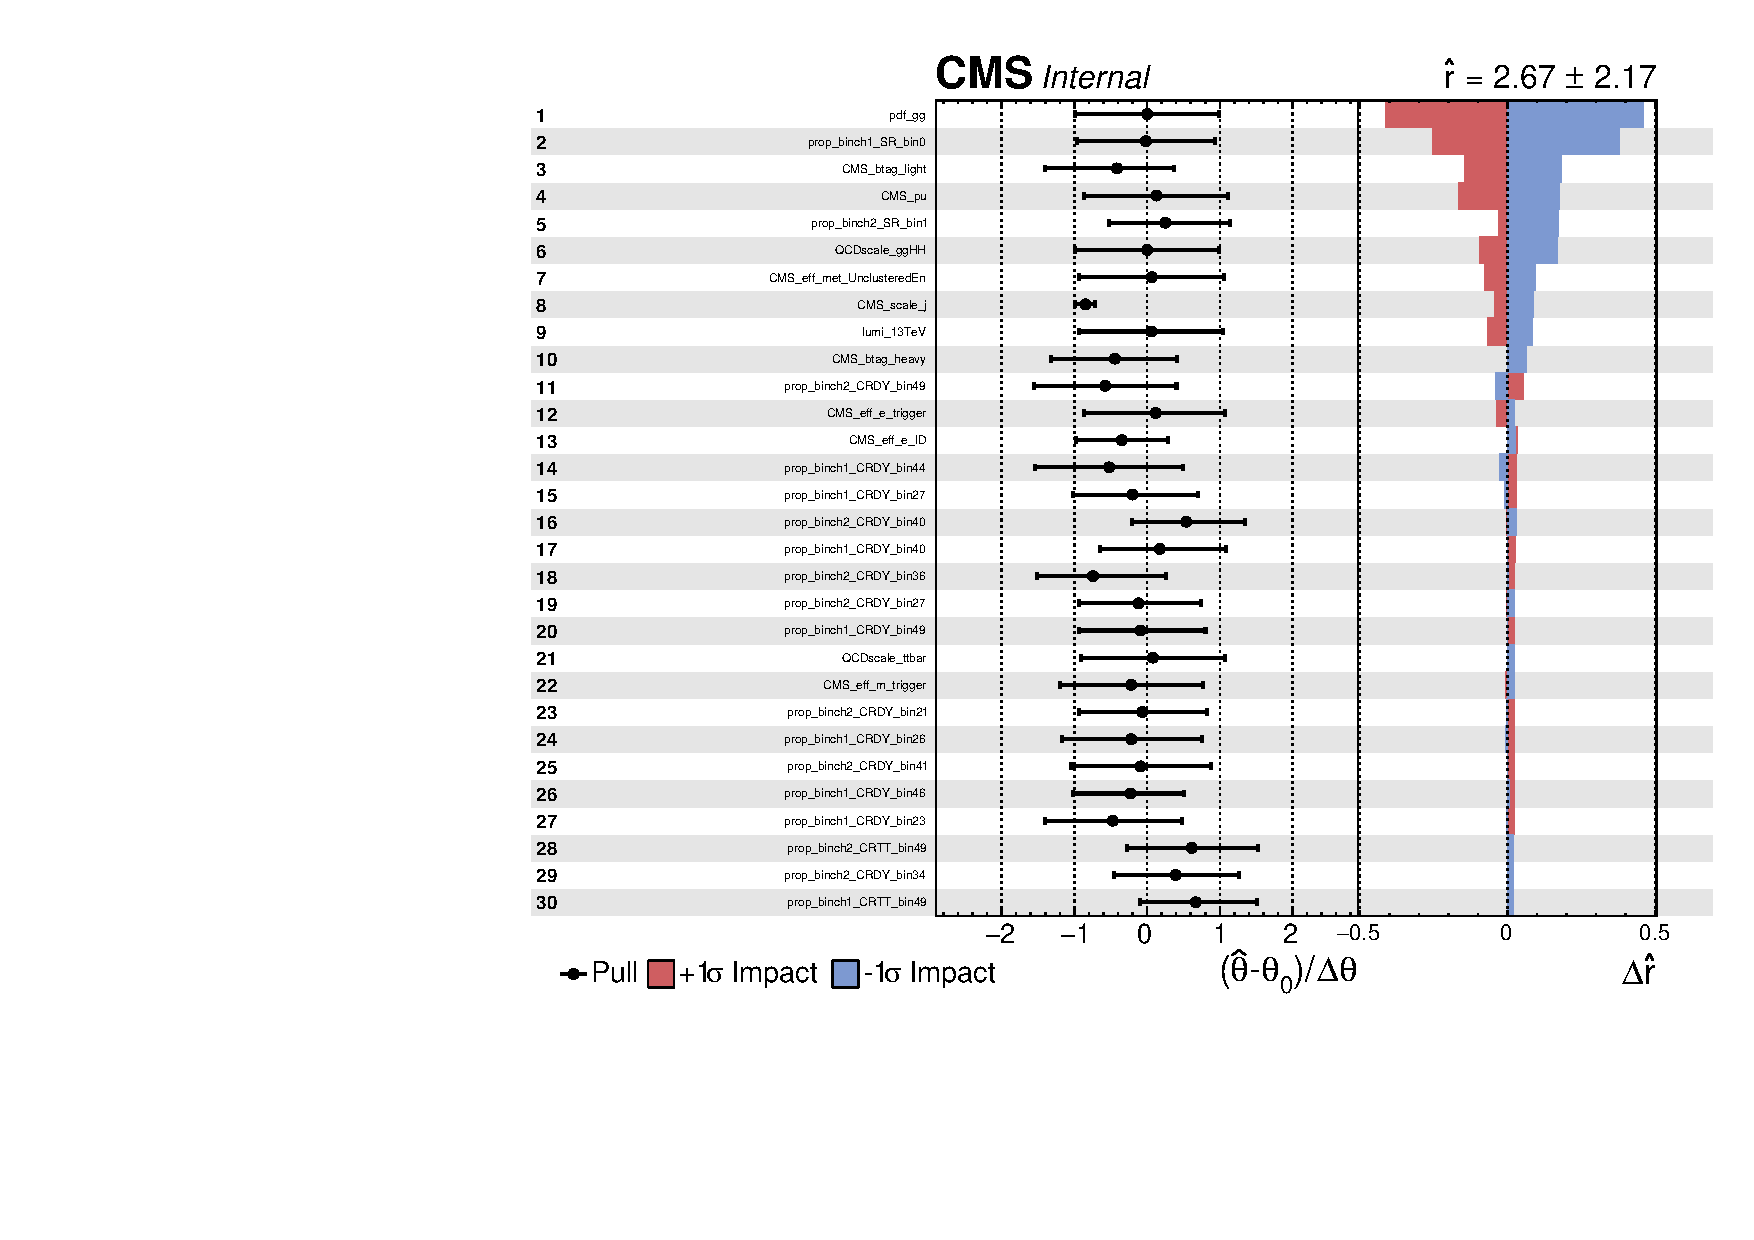
\includegraphics[width=0.5\textheight]{figures/impacts_50_strategy2_july23_300.pdf}
%% 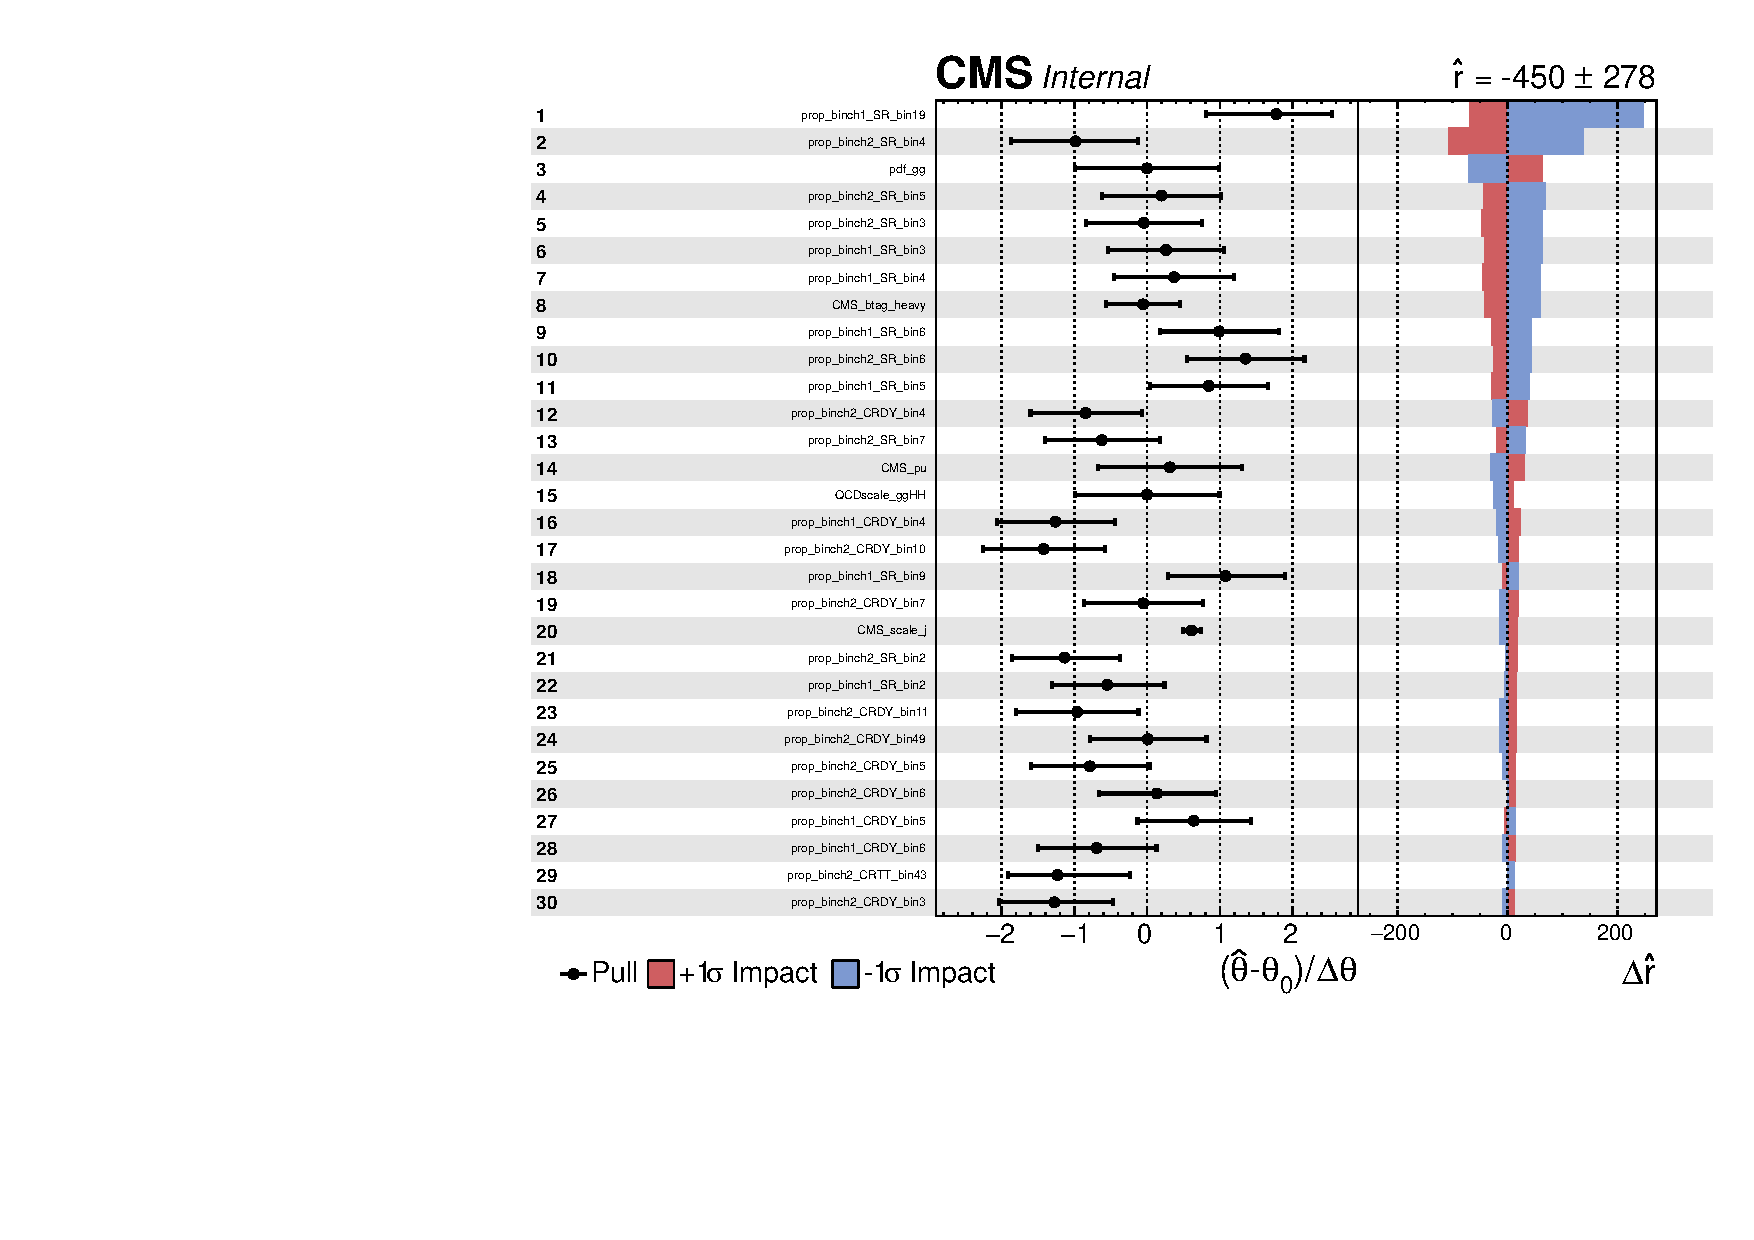
\includegraphics[width=0.5\textheight]{figures/impacts_1500_strategy0_july23_900.pdf}
%% \caption{ Impacts plot for 300(top) and 900 (bottom) GeV case.}% Actual limit at this mass point is $248.25_{-71.07}^{+103.9}$~pb.}
%% \label{fig:impactsBBB}
%% \end{figure}
%% \end{center}



%Following the Higgs PAG list of question for the preapproval checks ~\cite{HiggsPAGPreapprovalChecks}, we produce for 300 GeV case fit results for a background-only Asimov toy (Fig.~\ref{mlfit_Asimov}) and a signal+background Asimov toy (Fig.~\ref{mlfit_Asimov}), with the corresponding outputs of running "diffNuisances.py" that can be found at ~\cite{Comparison_of_nuisances_expectedSignal0_350} and ~\cite{Comparison_of_nuisances_expectedSignal1_350}. 





%\begin{table}
\begin{sidewaystable}
\begin{center}
\caption{Yield variations, ee channel, 300 GeV.}
\begin{tabular}{ | c | c | c | c | c | c |c | c | } \hline
 sample & b-tagging &  mistag &  electron IDnISO &  electron tracker &  electron trigger &  jet resolution &  jet scale \\\hline
  DY &              4.3 &     7.4 &              5.4 &               1.1 &               2.1 &             0.2 &        5.3 \\
  TT &              0.5 &     7.4 &              4.7 &               1.1 &               1.9 &             0.0 &        0.5 \\
  signal\_bbzz &    0.2 &     7.6 &              5.0 &               1.1 &               2.0 &             0.7 &        5.8 \\
  signal\_bbww &    0.0 &     7.6 &              6.7 &               1.1 &               2.9 &             0.0 &        1.6 \\\hline
\end{tabular}
\label{normalization_electron}
\end{center}
%---------------------------------------------------------------------                                        
%Vertical lines as column separators                                                                          
\begin{center}
\caption{Yield variations, mm channel, 300 GeV.}
\begin{tabular}{ | c | c | c | c| c | c | c | c| c |}\hline
sample &  b-tagging &  mistag &  muon ID &  muon ISO &  muon tracker &  muon trigger &  jet resolution &  jet scale \\\hline
  DY &              4.9 &     7.0 &      0.2 &       0.1 &           0.1 &           0.4 &             0.2 &        9.4 \\
  TT &              0.9 &     7.2 &      0.2 &       0.1 &           0.0 &           0.4 &             0.6 &        0.7 \\
  signal\_bbzz &    0.3 &     7.7 &      0.2 &       0.1 &           0.0 &           0.4 &             0.5 &        4.4 \\
  signal\_bbww &    0.0 &     9.2 &      0.2 &       0.1 &           0.0 &           0.1 &             0.0 &        8.5 \\\hline
\end{tabular}
\label{yieldVariations}
\end{center}
%\end{table}
\end{sidewaystable}


%The impacts plot with BBB uncertainties can be found at Fig.\ref{fig:impactsBBB}.%~\ref{pulls}.



%% \begin{center}
%% \begin{figure}[tbp]
%% \hfill\break 
%% \hfill\break 
%% \hfill\break 
%% \hfill\break
%% 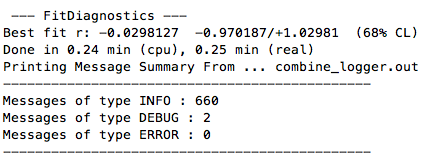
\includegraphics[width=0.4\textheight]{figures/expS0.png}
%%  \hfill\break
%%  \hfill\break
%% %\vspace{10mm} %10mm vertical space 
%% 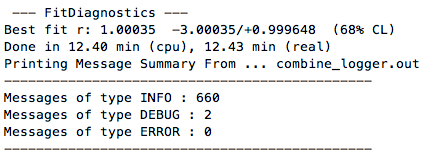
\includegraphics[width=0.4\textheight]{figures/expS1.png}
%% \caption{ Results of a background-only (top) and a signal+background Asimov toy fits (bottom). }
%% \label{mlfit_Asimov}
%% \end{figure}
%% \end{center}



%% \begin{center}
%% \begin{figure}[tbp]
%% 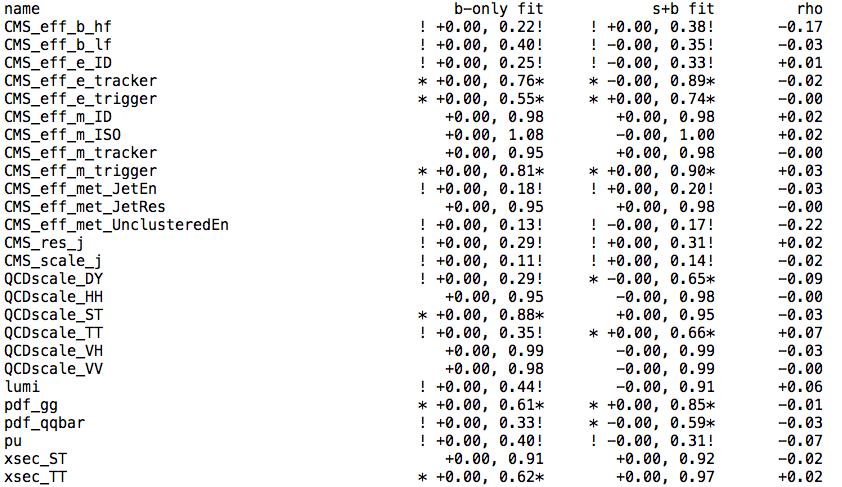
\includegraphics[width=0.6\textheight]{figures/diffNuisances_s0.png}
%%  \hfill\break
%%  \hfill\break
%% %\vspace{15mm} %15mm vertical space
%% 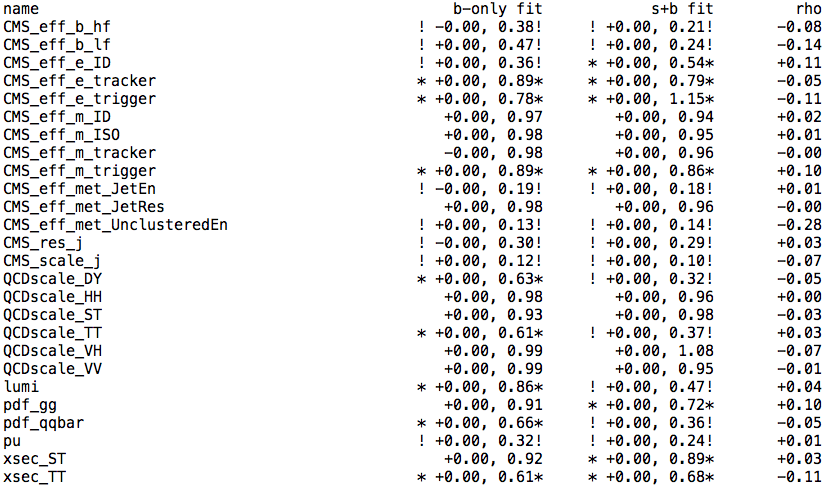
\includegraphics[width=0.6\textheight]{figures/diffNuisances_s1.png}
%% \caption{ Tables of nuisances, corresponding background-only (top) and a signal+background Asimov toy fits (bottom), as well as the correlation coefficient (rho) between each nuisance parameter and the signal strength (r).}
%% \label{diffNuisances}
%% \end{figure}
%% \end{center}




%% \begin{figure}[tbp]
%% \begin{center}
%% 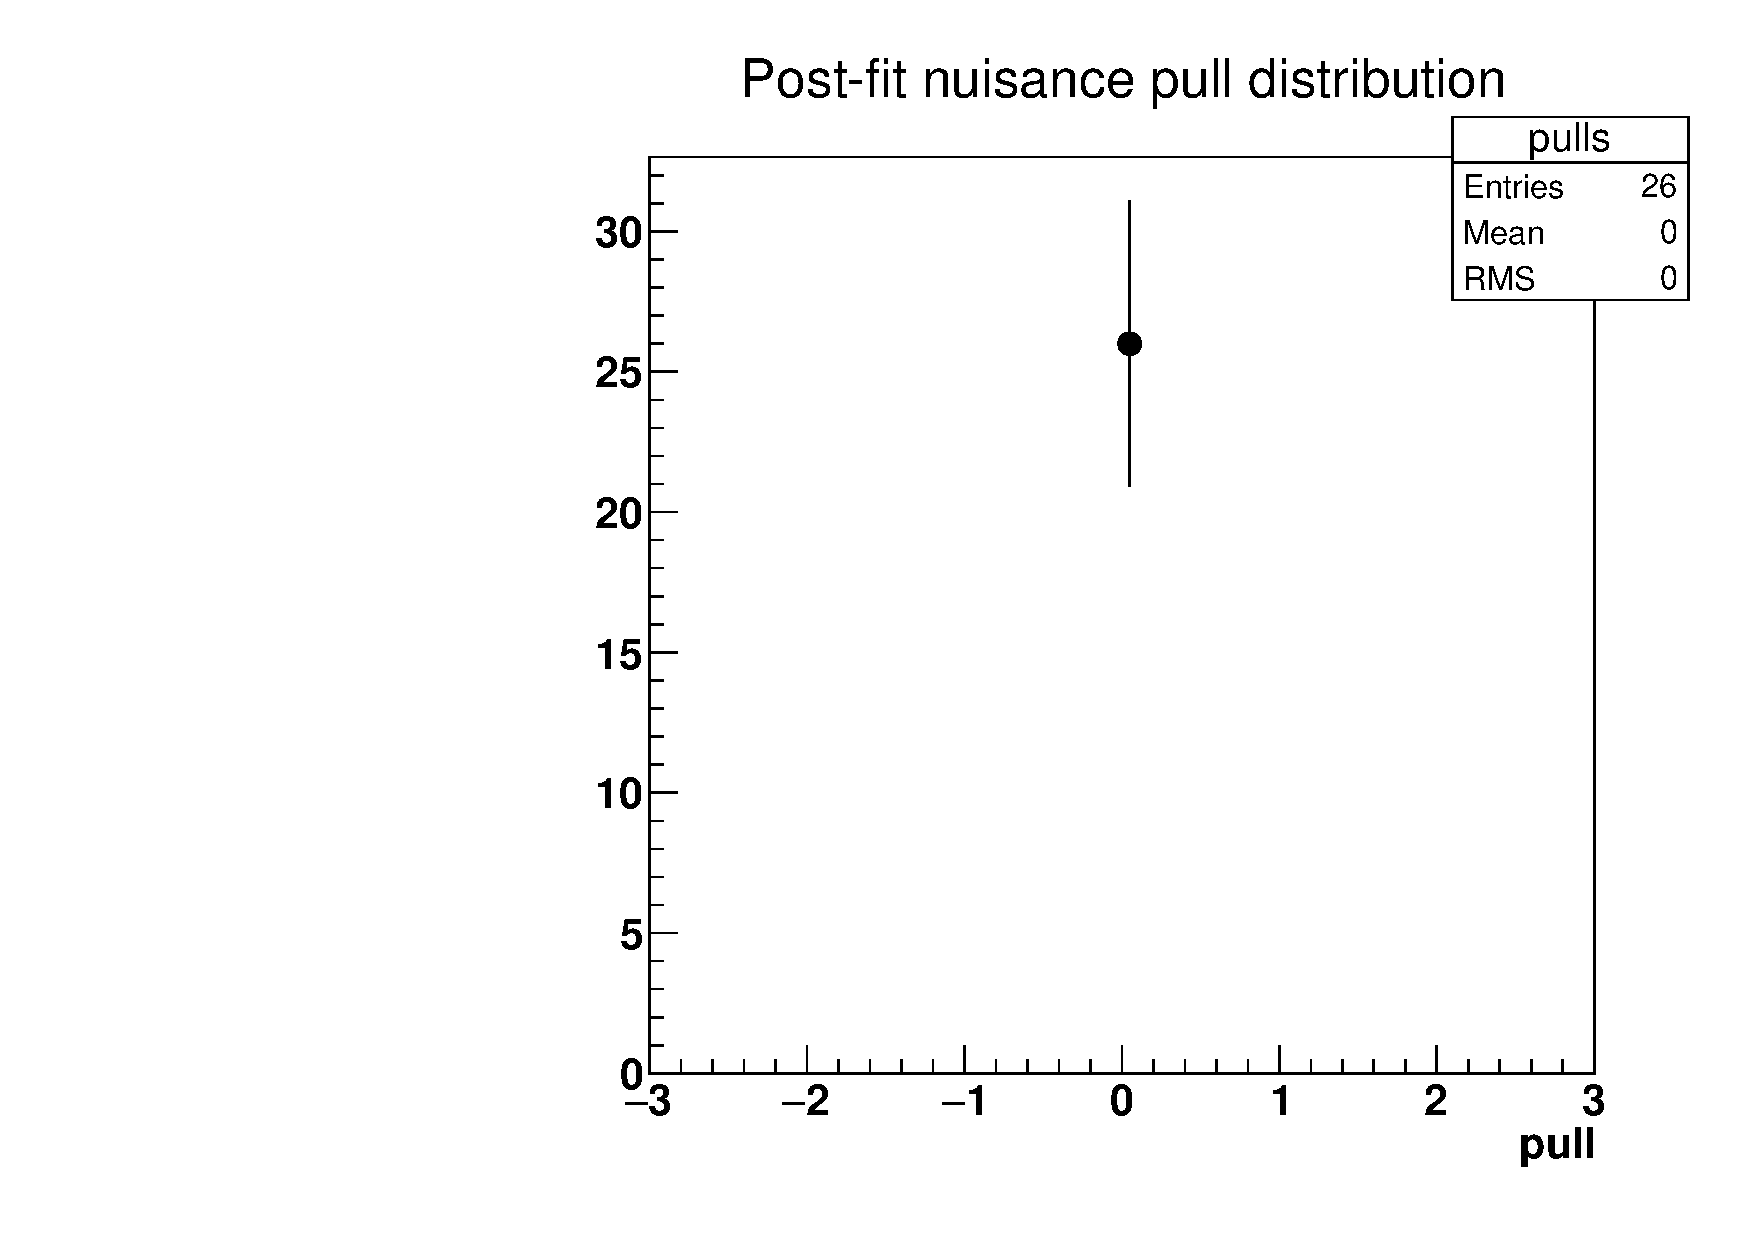
\includegraphics[width=0.5\textheight]{figures/pull_s0.pdf}
%% 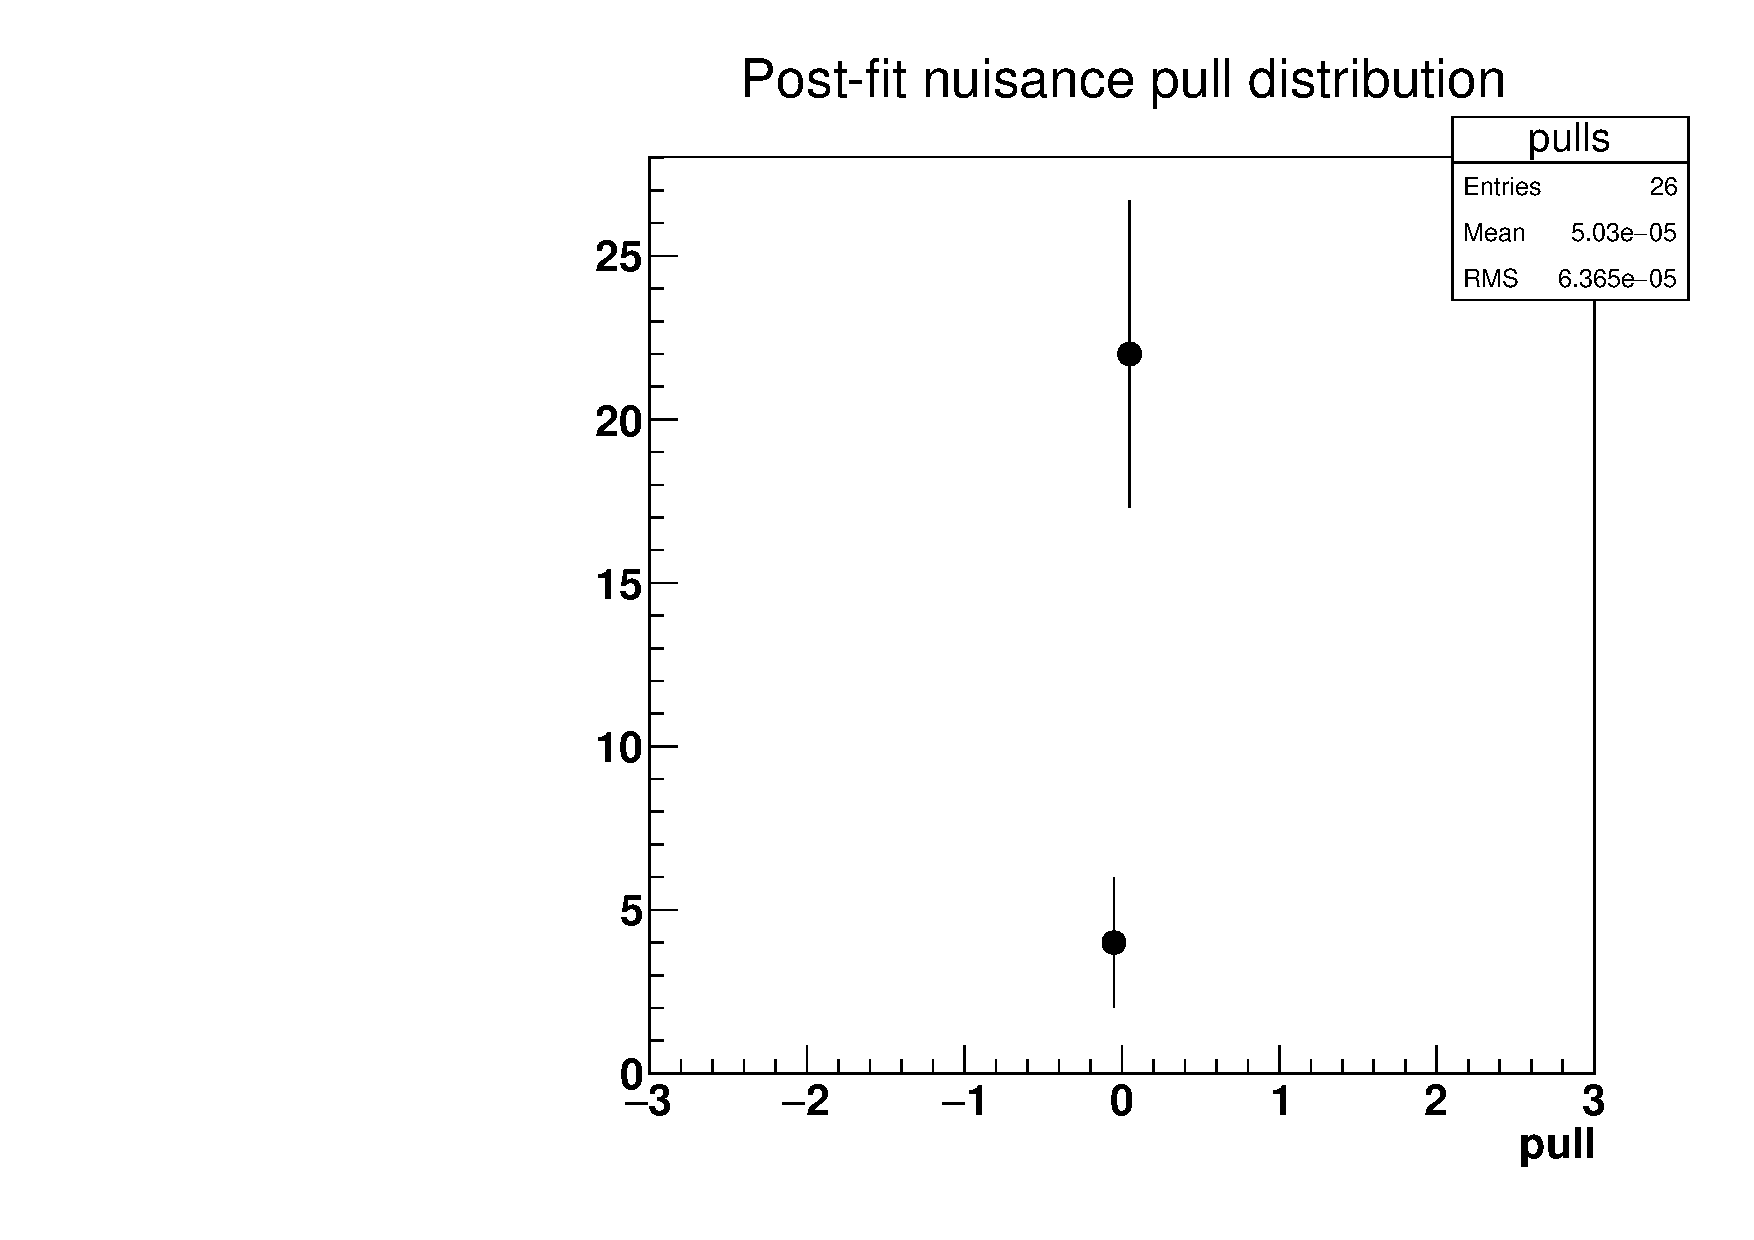
\includegraphics[width=0.5\textheight]{figures/pull_s1.pdf}
%% \caption{ Pulls plots for the background-only (top) and a signal+background Asimov toy fits (bottom).}
%% \label{pulls}
%% \end{center}
%% \end{figure}

